\documentclass{beamer}

%% Configuración de la presentación
\mode<presentation> {

  \usetheme{Warsaw}

  
  \usecolortheme{beaver}
 
}

%% Fuentes de tamaño arbitrario
\usepackage{lmodern}
\usepackage{amsfonts}
\usepackage{dsfont}


%% Gráficos
\usepackage{graphicx} % Allows including images
\usepackage{booktabs} % Allows the use of \toprule, \midrule and \bottomrule in tables

%%% Castellano.
% noquoting: Permite uso de comillas no españolas.
% lcroman: Permite la enumeración con numerales romanos en minúscula.
% fontenc: Usa la fuente completa para que pueda copiarse correctamente del pdf.
\usepackage[english,spanish,es-noquoting,es-lcroman]{babel}
\usepackage[utf8]{inputenc}
\usepackage[T1]{fontenc}
\selectlanguage{spanish}

\usepackage{tikz}
\usepackage{tikz-cd}
\usepackage{tikz-3dplot}

\usepackage{verbatim}
\usetikzlibrary{arrows,shapes}
\usepackage{amsthm}
\usepackage{accents}
\usepackage{amsmath,amssymb,lmodern}
\usepackage{fontawesome}
\usepackage{setspace}
\usepackage{subfig}
\usepackage{media9}
\usepackage{graphicx}
\usepackage{multimedia}


% Definitions
\theoremstyle{plain}
\newtheorem{thm}{Teorema}
\theoremstyle{definition}
\newtheorem{defn}[thm]{}
\theoremstyle{plain}
\newtheorem{prop}[thm]{}
\theoremstyle{definition}
\theoremstyle{remark}
\newtheorem{rem}[thm]{Nota}
\theoremstyle{definition}
\newtheorem{lem}[thm]{Lema}
\newtheorem{cor}[thm]{Corolario}
\newtheorem{ejemplo}[thm]{Ejemplo}
\newtheorem{ejemplos}[thm]{Ejemplos}
% Counter

\newcounter{saveenumi}
\newcommand{\seti}{\setcounter{saveenumi}{\value{enumi}}}
\newcommand{\conti}{\setcounter{enumi}{\value{saveenumi}}}

% Sections
\AtBeginSection{\frame{\sectionpage}}
\newtranslation[to=spanish]{Section}{Sección}

%comandos para agilizar la escritura de simbolos frecuentes
\newcommand{\sphere}{\mathds{S}^{d-1}}
\newcommand{\esfera}{\mathds{S}^{2}}
\newcommand{\orto}{\mathbb{O}^d}
\newcommand{\R}{\mathds{R}^d}
\newcommand{\spharm}{\mathds{Y}^d_n}
\newcommand{\sphint}{\int_{\sphere}}

\defbeamertemplate{section page}{mine}[1][]{%
  \begin{centering}
    {\usebeamerfont{section name}\usebeamercolor[fg]{section name}#1}
    \vskip1em\par
    \begin{beamercolorbox}[sep=12pt,center]{part title}
      \usebeamerfont{section title}\insertsection\par
    \end{beamercolorbox}
  \end{centering}
}

%----------------------------------------------------------------------------------------
%	TÍTULO
%----------------------------------------------------------------------------------------

\title[]{Análisis y monitorización de aplicaciones a través de plugins con Naemon} % The short title appears at the bottom of every slide, the full title is only on the title page

\author{Sofía Fernández Moreno} % Your name
\institute[UGR] % Your institution as it will appear on the bottom of every slide, may be shorthand to save space
{
  Universidad de Granada \\ % Your institution for the title page
  % Your email address
}
\date{Septiembre de 2019} % Date, can be changed to a custom date

% logo of my university
\titlegraphic{
	
\includegraphics[width=2cm]{imagenes/logo_ugr.jpg}
	
\includegraphics[width=2cm]{imagenes/etsiit_logo.png}
}


\begin{document}
% Spanish
\selectlanguage{spanish}
% Para tikz
\pgfdeclarelayer{background}\theoremstyle{definition}
\pgfsetlayers{background,main}
% Secciones
\setbeamertemplate{section page}[mine]

%% Diapositiva de título.
\frame{\titlepage}

%% Diapositiva de contenidos.
% Throughout your presentation, if you choose to use \section{} and \subsection{} commands,
% these will automatically be printed on this slide as an overview of your presentation
%\begin{frame}
%  \frametitle{Contenidos} % Table of contents slide, comment this block out to remove it
%  \tableofcontents
%\end{frame}


%----------------------------------------------------------------------------------------
%	PRESENTACIÓN
%----------------------------------------------------------------------------------------

%------------------------------------------------
\section{Objetivos del proyecto} % Sections can be created in order to organize your presentation into discrete blocks, all sections and subsections are automatically printed in the table of contents as an overview of the talk
%------------------------------------------------
\begin{frame}
	\frametitle{Mundo DevOps}
\centering
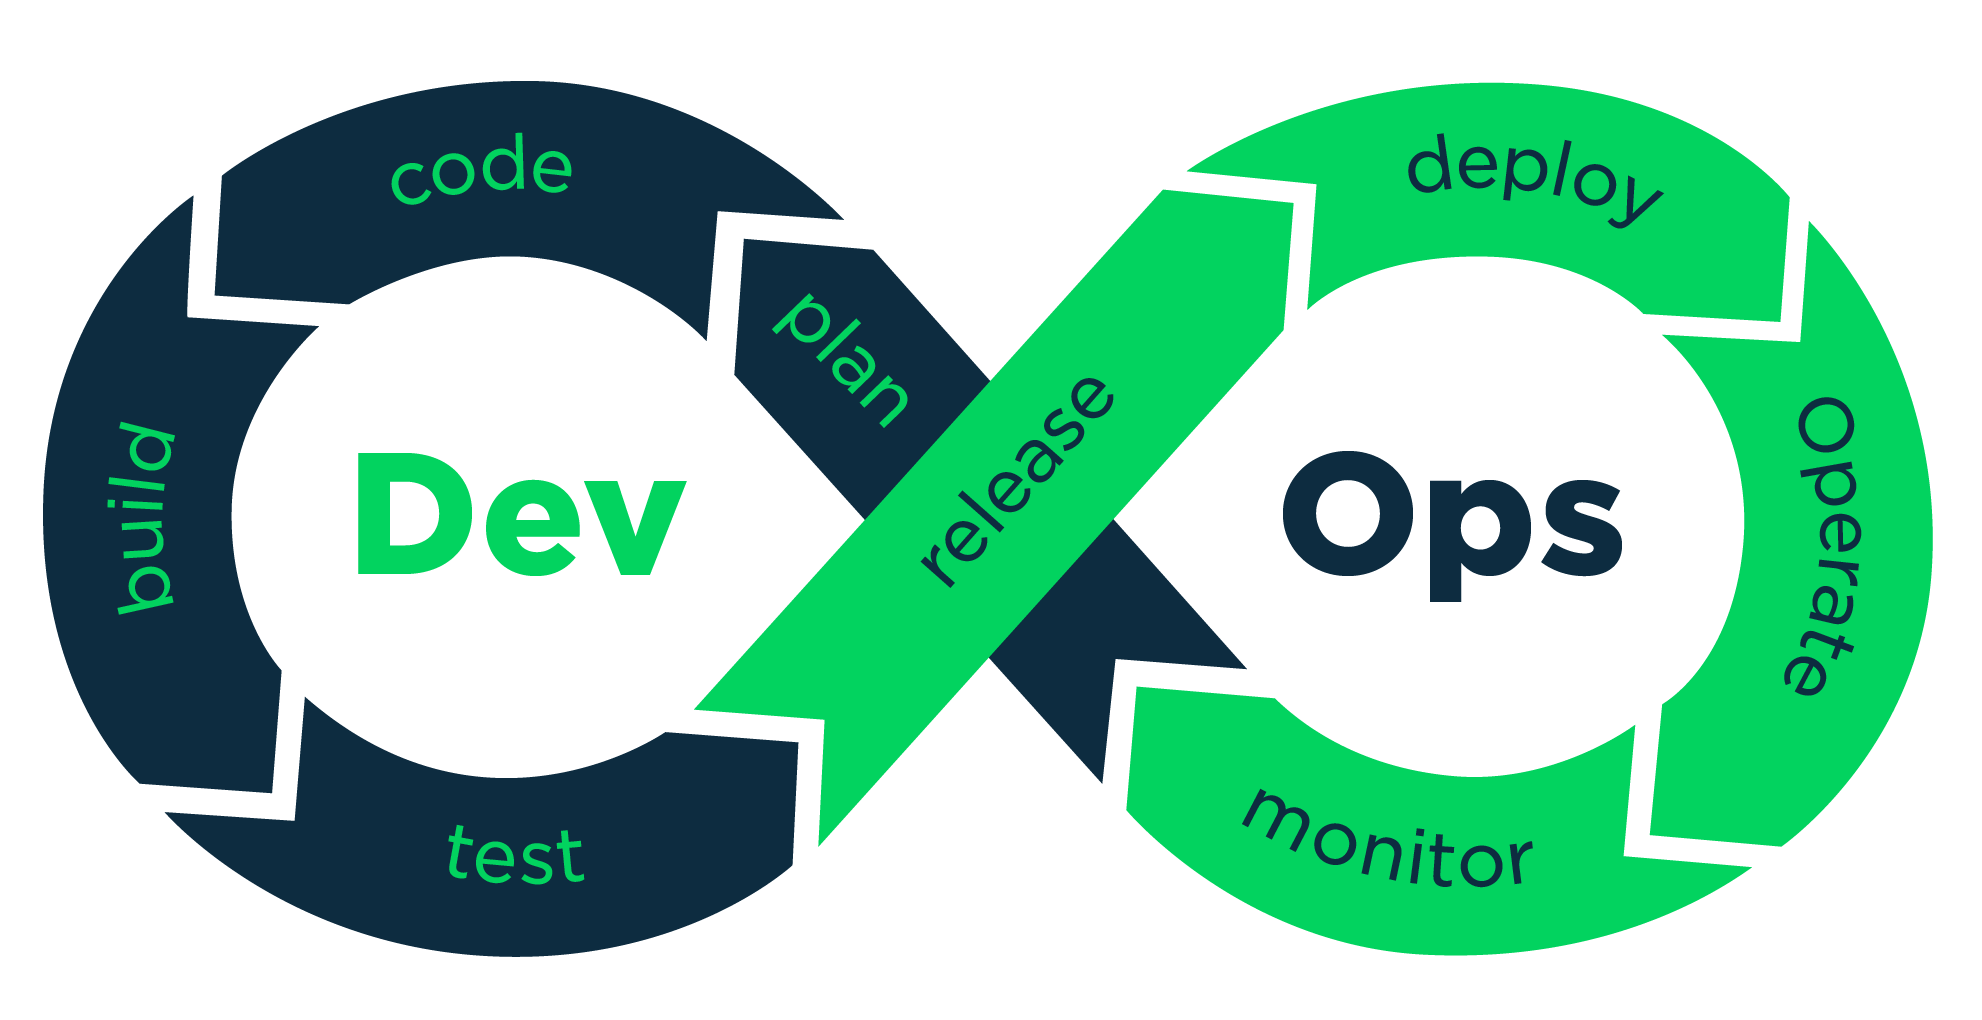
\includegraphics[scale=0.1]{imagenes/devops.png}	
\end{frame}
\section{Estado del arte}
\subsection{¿Qué es la monitorización?}
\begin{frame}
	\frametitle{¿Qué es la monitorización?}
	\begin{defn}
		La \textbf{monitorización} consiste en la manera de tomar las medidas preventivas y
		consecuentes con la información que se obtienen de todos los dispositivos
		que se encuentran conectados a una red, para evitar posibles eventos que
		hacen que se interrumpan el correcto funcionamiento de alguno de ellos
	\end{defn}
Dentro de este concepto es importante aplicar el uso del protocolo \textbf{SNMP} (Simple Network
Management Protocol).
\begin{prop}
	\textbf{SNMP} permite el intercambio de información amplia entre los diferentes dispositivos de red mediante consultas de forma remota (polling) y mediante mensajes basándose en eventos (traps).
\end{prop}

	
\end{frame}

\subsection{Comparativa herramientas de monitorización}
\begin{frame}
	\frametitle{Comparativa herramientas de monitorización}
	\centering
	
\includegraphics[scale=0.5]{imagenes/comparativaMonitorizacion.png}
\end{frame}

\subsection{Naemon}
\begin{frame}
	\frametitle{Archivo de configuración principal}
	\centering
	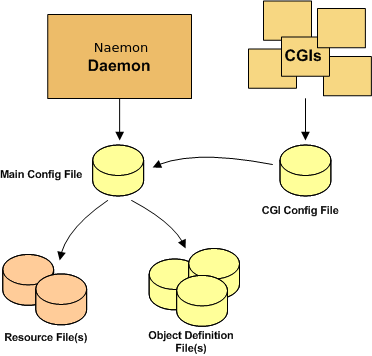
\includegraphics[scale=0.5]{imagenes/main_configuring.png}
		
\end{frame}

\begin{frame}
	\frametitle{Tipos de objetos}
	\begin{prop}
		La \textbf{configuración} de los distintos equipos y servicios a monitorizar se puede realizar a través de la carpeta \textbf{/etc/naemon/conf.d}
	\end{prop}
Podemos encontrar como objetos de definición:
\begin{itemize}
	\item Hosts
	\item Servicios
	\item Comandos
	\item Contactos
	\item Periodos de tiempo
\end{itemize}
	
\end{frame}

\begin{frame}
	\frametitle{
\includegraphics[width=1.5cm]{imagenes/thruk.png}}
	
	\centering
	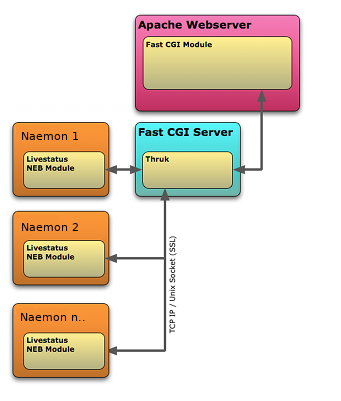
\includegraphics[scale=0.4]{imagenes/arquitecturaThruk.png}
	
\end{frame}
\begin{frame}
	\frametitle{Uso de plugins}
	\begin{block}
		
		Los \textbf{plugins} actúan como una capa de abstracción entre la lógica de supervisión presente en el demonio de Naemon y los servicios y hosts reales que se están supervisando.
	\end{block}
	\centering
	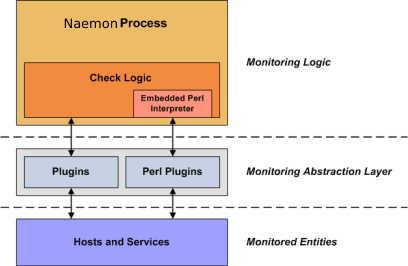
\includegraphics[scale=0.3]{imagenes/plugins.png}
	
	\begin{prop}
		El inconveniente de usar plugins en Naemon es que éste no tiene reflejo de qué es lo que está monitorizando, simplemente rastrea los cambios en el estado de esos recursos.
	\end{prop}
	
\end{frame}

\section{Realización del despliegue de Naemon} % Sections can be created in order to organize your presentation into discrete blocks, all sections and subsections are automatically printed in the table of contents as an overview of the talk
%------------------------------------------------


\subsection{Entorno de desarrollo}
\begin{frame}
	\frametitle{Uso de contenedores}
	\centering	
	
\includegraphics[scale=0.4]{imagenes/comparativaContenedores.png}
	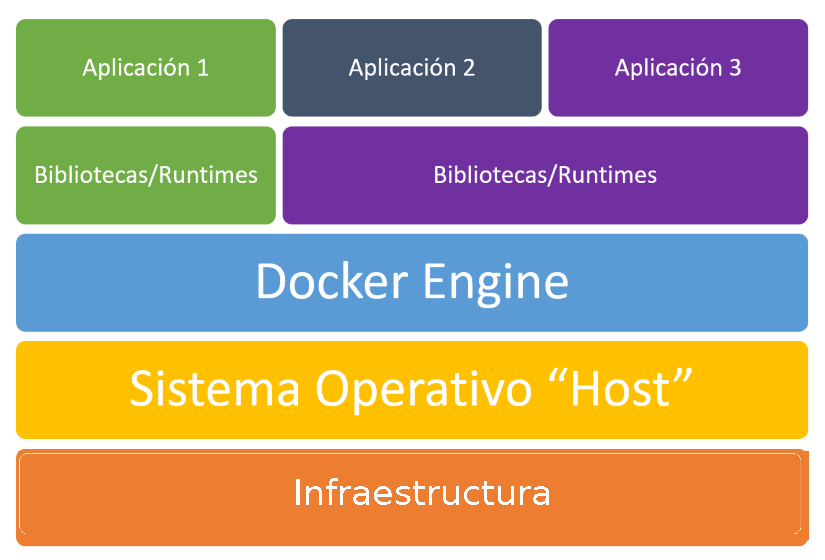
\includegraphics[scale=0.3]{imagenes/contenedores.png}
	
\end{frame}
\subsection{Desarrollo de despliegue}
\begin{frame}
	\frametitle{Creación de archivo Dockerfile}
	\begin{prop}
		
		Para poder realizar el despliegue tendremos que crear el fichero \textbf{Dockerfile}. Con este fichero construiremos la imagen de Naemon de forma automática, leyendo las instrucciones que le indiquemos.
	\end{prop}
	\centering
	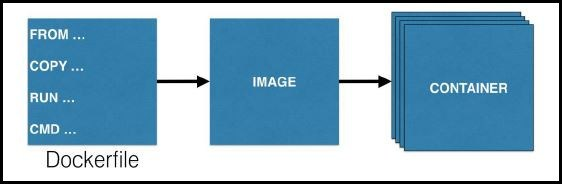
\includegraphics[scale=0.4]{imagenes/dockerfile-image.png}
	
\end{frame}



\begin{frame}
		\frametitle{Archivo de ejecución ENTRYPOINT (run.bash)}
	\centering
	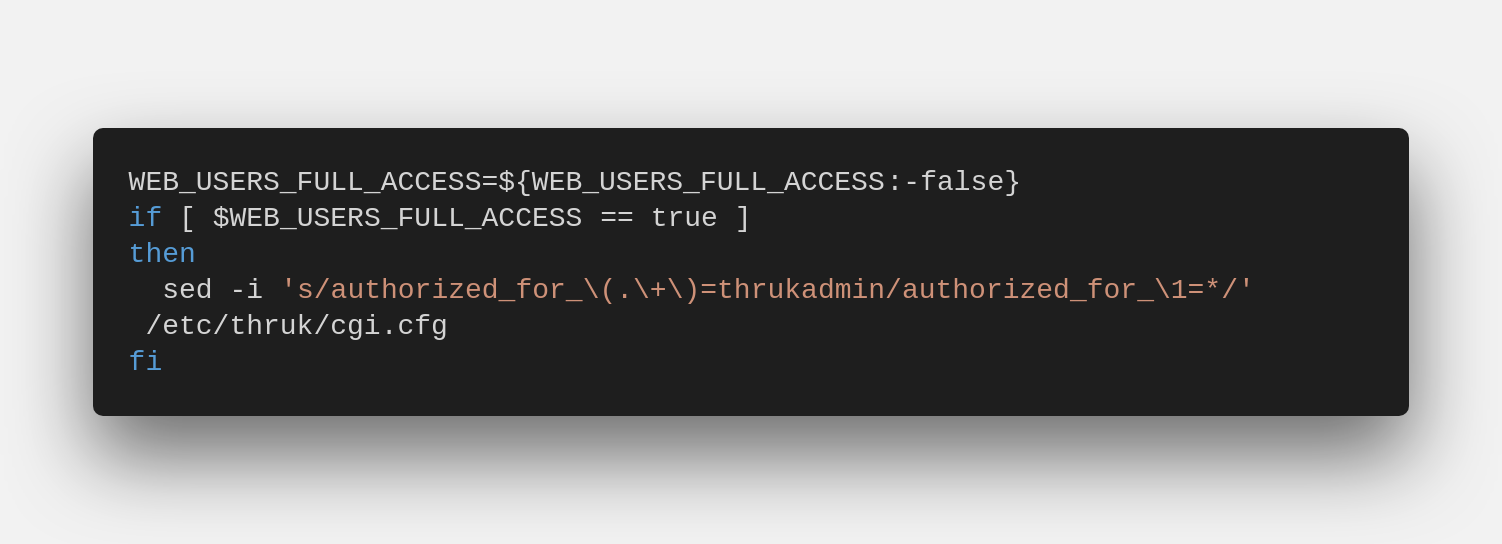
\includegraphics[scale=0.2]{imagenes/accesothrukadmin.png}
	
\end{frame}

\begin{frame}
	\frametitle{Orquestación de las aplicaciones}
	\begin{defn}
		La \textbf{orquestación} aplicada en este despliegue consiste en que el sistema requiere una configuración más
		manual de los recursos y no permite el escalado de forma muy eficiente.
	\end{defn}
\end{frame}
\begin{frame}
	\frametitle{Docker-Compose}
	Permite la orquestación estática orientada a un funcionamiento más centrado en un solo servidor, esta nos permite a través de un fichero YML, la definición y ejecución de aplicaciones Docker en múltiples contenedores.
	
	\centering
	
\includegraphics[scale=0.3]{imagenes/dockercompose.png}
\end{frame}
\section{Pruebas de carga} 
\begin{frame}
	\frametitle{Definición}
	\begin{defn}
	La \textbf{prueba de carga} se trata de una prueba que generalmente observa el comportamiento de una aplicación bajo una serie de peticiones.

\end{defn}
\end{frame}

\begin{frame}
	\frametitle{¿Sólo monitorizar?}
	Para este proyecto se ha elegido la opción de realizar \textbf{pruebas de carga} para poder simular el uso de concurrencia real en nuestro despliegue de Naemon.
	Además usaremos este tipo de prueba puesto que queremos medir la \textit{performance} o rendimiento de un sitio web, el cual mencionaremos más adelante y este tipo de prueba nos será de gran utilidad.
\end{frame}

\subsection{Comparativa de herramientas}
\begin{frame}
	\frametitle{Comparativa de herramientas}
	\centering
	
\includegraphics[scale=0.8]{imagenes/comparativaHerramientasPrueba.png}
	
\end{frame}

\subsection{Locust}
\begin{frame}
	\frametitle{Funcionamiento de Locust}
	Debemos activar el servidor web y luego para poder usar Locust debemos configurar un archivo \textbf{locustfile.py} que contará con el código necesario para realizar las pruebas de carga necesarias, distribuyendo la prueba de rendimiento en diferentes máquinas para que se
	pueda crear más carga en la aplicación.
	
\end{frame}
\begin{frame}
	\frametitle{Locustfile}
	\begin{itemize}
		\item \textbf{TaskSet}: se trata de una colección de tareas, es decir, define el comportamiento del usuario. Para cada acción definida debe definirse la anotación @task.
		\item \textbf{HttpLocust}: utilizada para cargar la prueba de rendimiento de un sistema en el servidor. Representa un usuario el cual será atacado y que será probado con carga. Dicha clase crea un atributo cliente que se trata del cliente HTTP que se encarga de realizar el enlace entre la
		sesión y las peticiones.
	\end{itemize}
\begin{center}
	
\includegraphics[scale=0.2]{imagenes/python.png}
\end{center}

\end{frame}
\begin{frame}
		\centering
	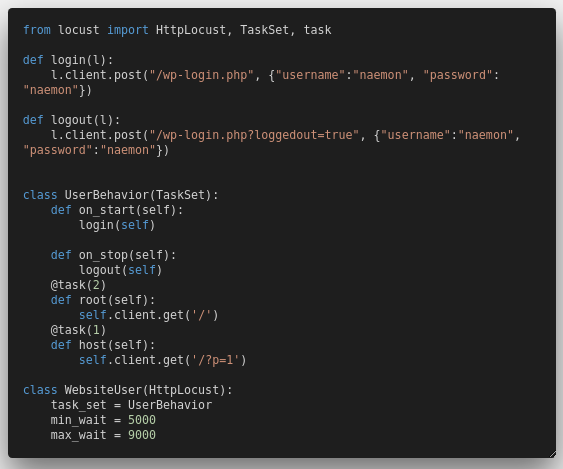
\includegraphics[scale=0.4]{imagenes/locustfile.png}
\end{frame}
\section{Pruebas de carga en un sistema} 

\subsection{Creación de archivo docker-compose}
\begin{frame}
	\frametitle{Estructura Docker-Compose}
	\centering
	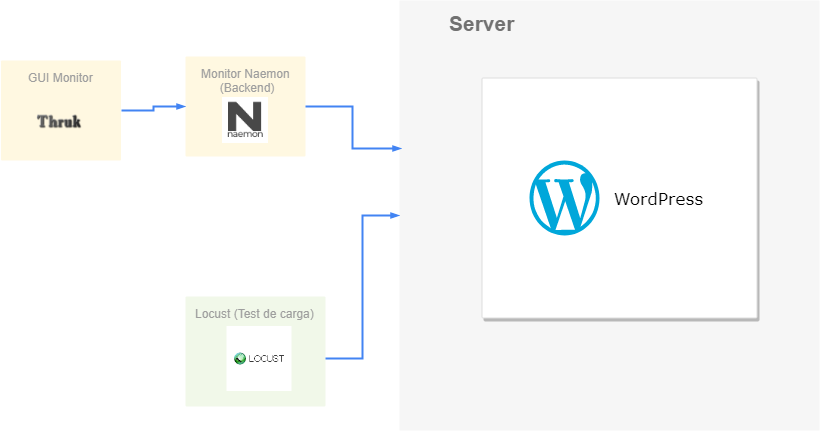
\includegraphics[scale=0.3]{imagenes/process.png}
\end{frame}
\subsection{Realización de pruebas}
\begin{frame}
	\frametitle{Enlazado con Locust}
	Para poder enlazar Locust con el sistema debemos adaptar la configuración interna del archivo \textbf{locust.config.json}. Este archivo será añadido al fichero \textbf{docker-compose.yml} junto al \textbf{locustfile.py}.
	Dicho archivo nos servirá para especificar la URL raíz de la API a la que se va a redirigir la API de Locust, junto con la lista de nombres de clase para las subclases de Locust que se usarán en la prueba.

	\centering
	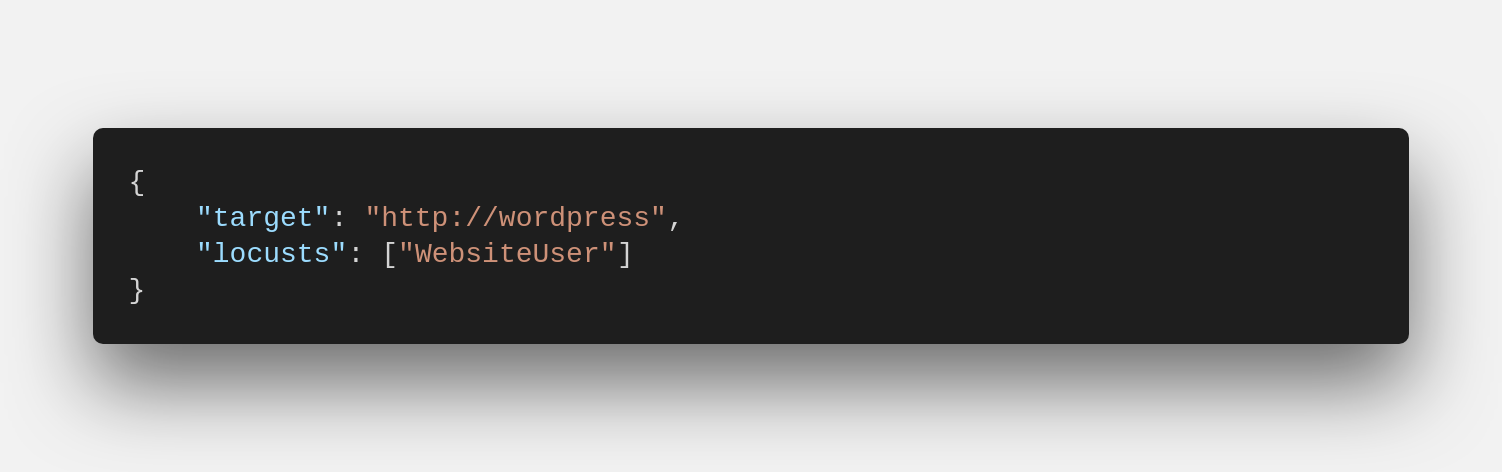
\includegraphics[scale=0.15]{imagenes/jsonLocust.png}
	\end{frame}
\begin{frame}
\frametitle{Interfaz de Locust}
\begin{itemize}			
	\item \textbf{Number of users simulate}: serán los números de usuarios que queremos asignar a la ejecución de las pruebas
	\item \textbf{Hatch rate}: representa por cada segundo, cuántos usuarios se agregarán a los usuarios actuales hasta la cantidad total de usuarios. Por cada hatch realizado Locust llama a la función on\_start si existe.
\end{itemize}
	
	\centering
	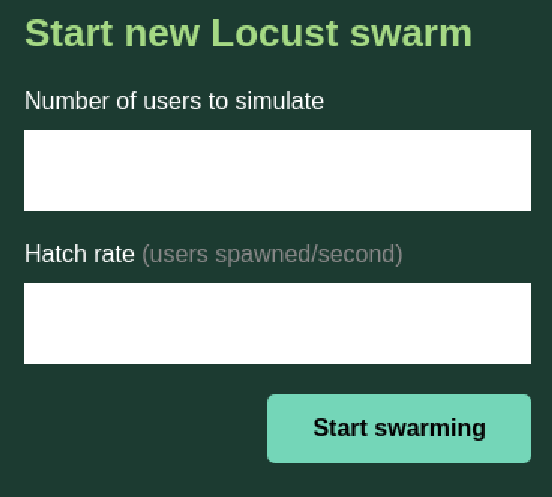
\includegraphics[scale=0.15]{imagenes/locustInterfaz.png}
\end{frame}

\begin{frame}
	\frametitle{Creación de host y servicios en Naemon}
	La carpeta /etc/naemon/conf.d/ cuenta con el siguiente contenido:
		
	\begin{center} 	
			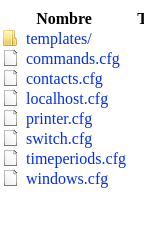
\includegraphics[scale=0.3]{imagenes/confd.png}
	\end{center}	
	Dentro de la carpeta templates se modificarán los archivos host.cfg, services.cfg para realizar las pruebas de rendimiento del sistema implementado en Naemon.
	
\end{frame}
\begin{frame}
	\frametitle{Creación de host y servicios en Naemon II}
	Añadiremos en el archivo \textbf{DockerFile} creado anteriormente las siguientes líneas:

	\centering
	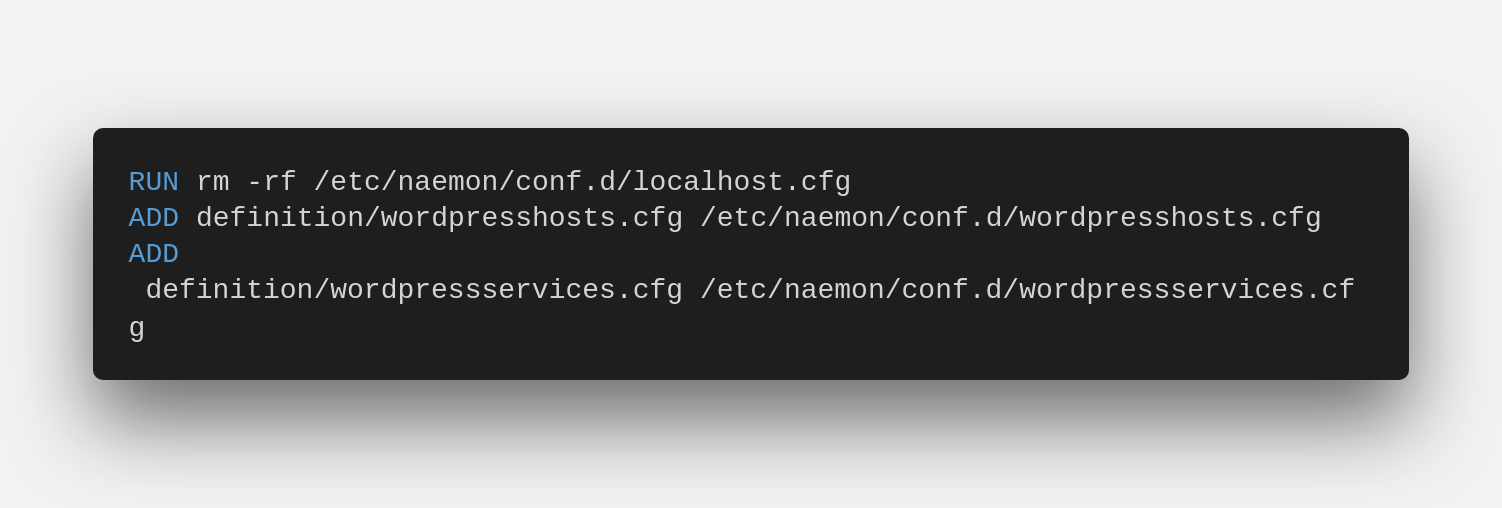
\includegraphics[scale=0.15]{imagenes/dockerfuileHOST.png}	
\end{frame}

\section{Modelado de las pruebas} % Sections can be created in order to organize your presentation into discrete blocks, all sections and subsections are automatically printed in the table of contents as an overview of the talk
%------------------------------------------------
\subsection{Carga de trabajo}
\begin{frame}
	\frametitle{¿Qué es la carga de trabajo?}
	\begin{defn}
		La \textbf{carga de trabajo} es el conjunto de todas las peticiones que el sistema recibe de su entorno
		durante un periodo de tiempo dado.
	\end{defn}
El análisis de la carga es un papel fundamental en cualquier
estudio en los que hay que determinar \textbf{índices de rendimiento}, estos se
encuentran directamente relacionados con la carga y no se pueden expresar
de forma independiente a ésta. Además el índice de rendimiento siempre debe
ir determinado de la información de la carga bajo la que fue determinado.
	
\end{frame}
\subsection{PNP4Nagios}

\begin{frame}
	\frametitle{PNP4Nagios en Dockerfile}
	\begin{defn}
		\textbf{PNP4Nagios} es un modulo para Naemon y además para
		Nagios que analiza los datos de rendimiento de los servicios que tengamos implementados en cada host, almacena automáticamente los datos en bases	de datos \textbf{RRD} (bases de datos Round Robin).
	\end{defn}
	\begin{center}
		
\includegraphics[scale=0.8]{imagenes/Pnp4nagios_logo.jpg}
	\end{center}

\end{frame}

\begin{frame}
	\frametitle{Exportación de datos en CSV}
	Para ello la API nos ofrece la forma de
	exportación a CSV de la siguiente forma:
	
	\textbf{$/pnp4nagios/xport/<format>?host=<hostname>\&srv=<servicedesc>$}
	\begin{itemize} 
	\item \textbf{$<format>$} especifica el formato de exportación, teniéndose la opción de XML, JSON y CSV.
	\item \textbf{$<hostname>$} especificaremos el nombre del host, en este caso introducimos el nombre wordpress.
	\item \textbf{$<servicedesc>$} especificaremos el servicio que queremos exportar su información.
	\end{itemize} 
\end{frame}
\begin{frame}
	\frametitle{Resultados}
\begin{frame}[plain]
	\movie[width=
	\paperwidth,borderwidth=10pt,poster,showcontrols]{
\includegraphics[width=\paperwidth]{imagenes/Pnp4nagios_logo.jpg}}{demo/demo.mp4}
\end{frame}

\end{frame}


\section{Conclusiones y futuros trabajos}

\begin{frame}
	
	\Huge{\centerline{Conclusiones}}
	
\end{frame}
\subsection{Trabajos futuros}
\begin{frame}
	\frametitle{Trabajos futuros}
	\centering
	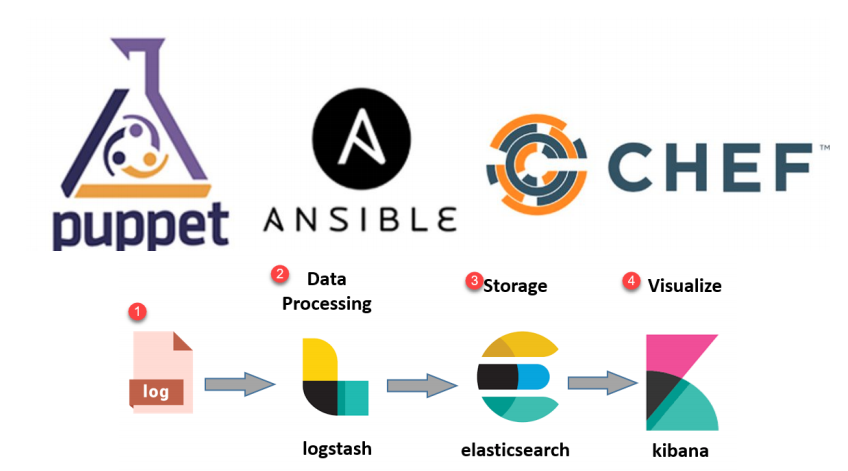
\includegraphics[scale=0.3]{imagenes/futuro.png}
	
\end{frame}
\subsection{}
\begin{frame}{}{}
	\Huge{\centerline{Gracias por su atención}}
	\centerline{\Huge{\raisebox{-.25\height}\faGithub}~\large{\href{https://github.com/sofiafernandezmoreno/TFG}{\alert{sofiafernandezmoreno/TFG}}}}

\end{frame}
\end{document}